\documentclass[conference]{IEEEtran}
\usepackage{cite}
\usepackage{amsmath,amssymb}
\usepackage{graphicx}
\usepackage{booktabs,tabularx,array}
\usepackage{xcolor}
\usepackage{tikz}
\usetikzlibrary{matrix,arrows.meta,positioning}
\usepackage[hidelinks]{hyperref}
\urlstyle{same}
\newcolumntype{Y}{>{\raggedright\arraybackslash}X}

\newcommand{\todo}[1]{\textcolor{red}{\textbf{[#1]}}}

\begin{document}

\title{Class-Aware Augmentation Selection for Multi-Class Object Detection}
\maketitle

% \begin{abstract}
% Written last (Stage 7).
% \end{abstract}

\begin{IEEEkeywords}
augmentation policy, data augmentation, gradient alignment, infrastructure inspection, multi-class images, object detection
\end{IEEEkeywords}

\section{Introduction}
\label{sec:intro}

Object detectors are increasingly used to automate visual inspection, where they must locate and classify several kinds of damage in the same image, such as cracks and potholes on roads or corrosion and cracking on bridges~\cite{shang2024automated,zheng2024deep,vision2025inspection}. Achieving reliable detection in these settings remains challenging, because the appearance of each damage type varies with illumination, surface texture, camera viewpoint and image quality, and a training set rarely covers this variation in full. The difficulty is compounded by differences among the categories themselves. Some are defined mainly by shape, such as thin longitudinal and transverse cracks~\cite{arya2024rdd}, whereas others are defined mainly by colour, such as rust and efflorescence on concrete~\cite{flotzinger2024dacl10k}. Consequently, improving detection in such settings requires exposing the detector to a wider range of visual conditions while preserving the cues that distinguish each category.

Data augmentation addresses the first part of this requirement by applying controlled edits, such as geometric, colour and image-quality transformations, to training images, so that the detector learns from more varied conditions without additional annotation. The effectiveness of an edit, however, depends on whether it preserves the cues that define each category. Colour jitter, for example, alters the very property that identifies rust while leaving the geometry of a crack intact, whereas Gaussian blur can erase a hairline crack while barely changing a pothole. The same edit can therefore provide useful variation for one category while removing essential information from another. In detection, this tension arises within a single training image rather than only between images: standard pipelines edit the whole image, so every object in it receives the same edit, and an edit that helps the detector learn one category can hinder another category in the same image. Such conflicts are easily overlooked, because augmentation is usually judged by accuracy averaged over classes, and gains in average accuracy can coexist with losses for individual classes~\cite{kirichenko2023}. This motivates augmentation that accounts for how each class responds to each edit, and that chooses the edit for an image according to the classes the image contains.

Existing augmentation methods have progressively moved toward this goal, but each stops short of it. AutoAugment and RandAugment search for or simplify one policy shared by the whole dataset~\cite{cubuk2019auto,cubuk2020rand}, and detection-specific extensions add edits restricted to annotated boxes or adapt the policy to object scale~\cite{zoph2020det,chen2021scale}; none of these policies, however, depends on the category of the objects being edited. Class-aware approaches recognize that categories may require different augmentations~\cite{tsuchiya2019,yoo2023,cheung2022adaaug}, and road-damage detection work has varied augmentation probabilities by damage type~\cite{rdd_detectron2}. Because these policies are fixed before or apart from detector training, they cannot follow changes in what each class needs as learning progresses. Online methods remove this restriction by adapting augmentation from the feedback of the evolving model, but the feedback they use introduces two further limitations. Tolerance-based controllers such as CTAugment and CUDA adjust augmentation according to whether the model still recognizes augmented examples~\cite{berthelot2020,ahn2023cuda}, which indicates what the model can already handle rather than whether training on the edit improves it. Benefit-based methods such as BDA, DDAS and MADAug measure that improvement through a held-out loss~\cite{lu2023bda,liu2021ddas,hou2023madaug}, but they compute it over all classes together, so an edit that helps frequent classes can be preferred even when it harms a rare one. Moreover, the class-aware methods among them are formulated for classification, where each training sample carries one label, and therefore do not specify which class should govern an image that contains several.

This gap matters in detection because the classes in one image can disagree. A detector may learn well from blurred images of potholes while the thin cracks in the same images lose the structure that identifies them. A policy guided by pooled feedback sees only the net effect of blur and may apply it to both, whereas a policy keyed to a single class must ignore the other. What is needed instead is a measure of how much each edit helps each class learn, combined into one decision for the image that respects every class it contains.

To meet this need, we propose Class-Utility Augmentation (CUA), an online augmentation policy that selects the edit for each training image from the classes present in it. CUA is built around the \emph{class utility} of an edit, defined as the estimated amount that the edit helps a given class learn. CUA estimates this utility during training with a first-order argument from training-influence analysis~\cite{pruthi2020tracin}: if a gradient step on the edited image would reduce a class's loss on a held-out \emph{reference set} more than a step on the original image would, the edit currently benefits that class. For each training image, CUA then averages the utilities of the classes present, removes any edit that is reliably harmful to one of them, and samples a single edit from the remainder, with ``no edit'' always available as a candidate of zero utility (Fig.~\ref{fig:teaser}). Because the utilities are re-estimated from the current detector, the preferred edits can change as training proceeds, and because CUA requires no policy network and no separate search phase, it adds only a periodic gradient computation to standard training.

The value of CUA rests on the premise that classes respond differently to the same edit, so we examine this premise before evaluating the method. Across road damage (RDD2022), bridge damage (dacl10k) and everyday objects (PASCAL VOC)~\cite{everingham2010voc}, and with two detector families, Faster R-CNN~\cite{ren2017faster} and RetinaNet~\cite{lin2017focal}, we train detectors with one edit at a time to measure its effect on each class, and with an edit applied only to the objects of one class to separate its direct effect on that class from its effect on the others. We then compare CUA with shared-utility augmentation, an otherwise identical policy that averages utility over all classes, so that any difference between the two reflects class information alone. \todo{One-sentence summary of findings: which edits affect classes in opposite directions; CUA minus shared-utility on test macro AP50 with 95\% intervals; rank agreement between estimated utilities and measured effects.} In summary, this paper makes the following contributions:

\begin{enumerate}
    \item Class-Utility Augmentation, an online augmentation policy for multi-class object detection that estimates how much each edit helps each class learn and selects one edit per image from the classes it contains, with a no-edit option and a per-class harm block.
    \item A controlled measurement of how individual edits affect each class in detection, across three domains and two detector families, which also separates the effect of an edit on the class it is applied to from its effect on the other classes in the image.
    \item A comparison with a shared-utility counterpart that differs from CUA only in class information, together with standard augmentation baselines, and a test of whether the estimated class utilities agree with the measured per-class effects.
\end{enumerate}

\begin{figure}[t]
\centering
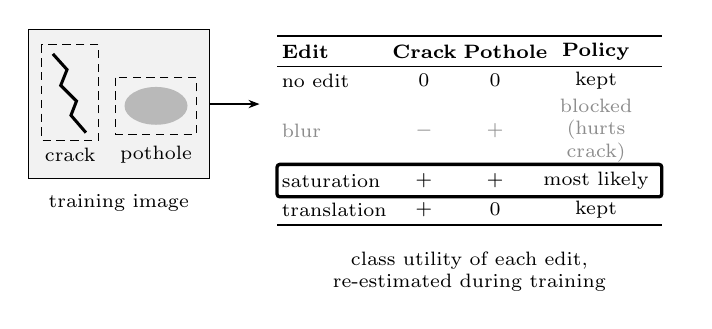
\begin{tikzpicture}[font=\scriptsize, >={Stealth[length=4pt]}]
  % schematic training image with two objects
  \node[draw, fill=gray!10, minimum width=2.3cm, minimum height=1.9cm, anchor=north west, inner sep=0pt] (img) at (0,0) {};
  \draw[line width=1.1pt] (0.32,-0.32) -- (0.5,-0.52) -- (0.42,-0.72) -- (0.62,-0.92) -- (0.55,-1.1) -- (0.74,-1.32);
  \draw[densely dashed] (0.18,-0.2) rectangle (0.9,-1.42);
  \node at (0.54,-1.6) {crack};
  \fill[gray!55] (1.63,-0.98) ellipse (0.4 and 0.24);
  \draw[densely dashed] (1.12,-0.62) rectangle (2.14,-1.34);
  \node at (1.63,-1.6) {pothole};
  \node[below=2pt of img, align=center] {training image};
  % per-class utility table (illustrative signs)
  \matrix (m) [matrix of nodes, anchor=north west, row sep=0pt, column sep=0pt,
      nodes={inner sep=1.5pt, minimum height=0.37cm, anchor=center},
      column 1/.style={nodes={text width=1.3cm, align=left}},
      column 2/.style={nodes={text width=0.8cm, align=center}},
      column 3/.style={nodes={text width=0.8cm, align=center}},
      column 4/.style={nodes={text width=1.55cm, align=center}},
      row 3/.style={nodes={text=black!45}}] at (3.05,0.02) {
    \textbf{Edit} & \textbf{Crack} & \textbf{Pothole} & \textbf{Policy} \\
    no edit     & $0$ & $0$ & kept \\
    blur        & $-$ & $+$ & blocked (hurts crack) \\
    saturation  & $+$ & $+$ & most likely \\
    translation & $+$ & $0$ & kept \\
  };
  \draw[thick] (m-1-1.north west) -- (m-1-4.north east);
  \draw (m-1-1.south west) -- (m-1-4.south east);
  \draw[thick] (m-5-1.south west) -- (m-5-4.south east);
  \draw[very thick, rounded corners=1pt] ([yshift=0.4pt]m-4-1.north west) rectangle ([yshift=-0.4pt]m-4-4.south east);
  \draw[->] (img.east) -- ([xshift=-3pt]img.east -| m.west);
  \node[below=3pt of m, align=center, text width=5.2cm] {class utility of each edit,\\ re-estimated during training};
\end{tikzpicture}
\caption{The idea behind CUA (illustrative signs, not measured values). The image contains a crack and a pothole. For each candidate edit, CUA keeps an estimate of how much the edit currently helps each class learn: its class utility ($+$ helps, $-$ hurts, $0$ no effect). Blur is removed because it reliably hurts the crack, although it helps the pothole. The remaining edits, including no edit, are sampled according to their utility averaged over the two classes, so saturation, which helps both, is the most likely choice. A policy shared across classes sees only the average over all classes and can still apply blur.}
\label{fig:teaser}
\end{figure}

\section{Related Work}
\label{sec:related}

\noindent\textbf{Augmentation policies for object detection.} Automatic augmentation began by treating the choice of edits as a search over a whole dataset. AutoAugment searches over operations, probabilities and magnitudes with validation accuracy as the reward~\cite{cubuk2019auto}; because this search is expensive, RandAugment reduces it to two shared parameters~\cite{cubuk2020rand}, and TrivialAugment goes further, showing that sampling one edit and strength uniformly at random is a strong baseline that needs no tuning~\cite{muller2021trivial}. Detection raises an additional question, namely where in the image an edit should act. Zoph \emph{et al.} answer it by learning policies that include edits restricted to the content of each box~\cite{zoph2020det}, Scale-Aware AutoAug by conditioning image- and box-level policies on object scale~\cite{chen2021scale}, and InterAug by constructing a tuning-free detection policy~\cite{thopalli2023interaug}. Inspection work has followed the same pattern with recipes designed for damage imagery, such as bounding-box augmentation combined with samples from generative adversarial networks~\cite{aghayan2024} or content- and perspective-aware cut-and-paste of damage~\cite{rdd_cutpaste}. Although these methods differ in how the policy is found, they share one property: the edit for an image is drawn from a single distribution, conditioned at most on location or scale, which implicitly assumes that every class benefits from the same edits.

\noindent\textbf{Class-aware augmentation.} Evidence from recognition suggests that this assumption does not always hold. Kirichenko \emph{et al.} show that augmentation which raises average ImageNet accuracy can lower the accuracy of individual classes~\cite{kirichenko2023}, and Tsuchiya \emph{et al.} find that augmentation methods for road-damage classification differ in their effect on individual damage classes~\cite{tsuchiya2019}. Several methods have therefore made augmentation depend on the class. Yoo and Kang derive class-specific parameters from a classifier trained beforehand~\cite{yoo2023}, AdaAug learns class-adaptive policies in a separate search~\cite{cheung2022adaaug}, CUDA updates a severity for each class during training~\cite{ahn2023cuda}, and Pham \emph{et al.} set augmentation probabilities for each damage type from an exploration of the data~\cite{rdd_detectron2}. These methods share a limitation that becomes decisive in detection. The classification methods select the augmentation by the label of a sample, which has no answer when an image contains objects of several classes, while the detection recipe sidesteps the question by fixing its probabilities before training. PSIS, the closest detection counterpart, adapts to per-class detection accuracy during training, but it controls how many instance-switched samples each class receives rather than which edit each image receives~\cite{wang2019psis}. A method for multi-class detection must therefore choose edits from the whole set of classes in an image, and must do so as the needs of the detector change during training.

\noindent\textbf{Adapting augmentation during training.} Online methods make this second requirement possible by updating augmentation from the model as it trains, but they differ in the feedback they treat as evidence that an edit is useful. Tolerance-based methods ask whether the current model still recognizes, or tolerates, augmented examples. CTAugment adjusts per-operation magnitudes from predictions on augmented labeled data, pooled over classes~\cite{berthelot2020}; CUDA raises or lowers the severity of each class according to how well its augmented examples are recognized~\cite{ahn2023cuda}; and TeachAugment keeps learned transformations recognizable to a teacher while making them hard for the target model~\cite{suzuki2022teach}. Recognition, however, reflects what the model can already handle rather than what it gains from training on the edit, which is the quantity augmentation is meant to increase. Benefit-based methods measure this gain more directly. BDA rewards an augmentation by the training gain it yields over a paired unaugmented reference~\cite{lu2023bda}, DDAS uses a one-step gradient update to estimate how the augmentation distribution affects a held-out loss, including for detection~\cite{liu2021ddas}, MADAug learns an input-dependent policy through a bilevel validation objective~\cite{hou2023madaug}, and RangeAugment and AdaAugment adapt magnitudes from task-loss feedback~\cite{mehta2022rangeaugment,yang2025adaaugment}. Their common limitation is that the benefit is computed over all classes together, so a gain for frequent classes can outweigh a loss for a rare one, which is precisely the trade-off that a multi-class image creates. Estimating the gain separately for each class need not be costly. TracIn measures the influence of a training example on a test loss through the alignment of their gradients~\cite{pruthi2020tracin}, and CUA applies the same first-order argument to edited versus unedited images and to a separate reference loss for each class.

Table~\ref{tab:policies} places these methods on two axes: the signal that guides augmentation, and whether that signal is resolved by class. Each ingredient of CUA has a precedent among them, including class conditioning, online adaptation, benefit signals and gradient-alignment estimates. None of them, however, keeps a benefit estimate separate for each class and combines these estimates into one decision for an image that contains several classes, with leaving the image unedited as an explicit option. CUA is designed for this case, and its comparison with shared-utility augmentation, which removes the class information and nothing else, tests whether the class information matters.

\begin{table*}[t]
\caption{Augmentation Methods Grouped by Feedback Signal and Class Resolution}
\label{tab:policies}
\centering
\small
\setlength{\tabcolsep}{3.5pt}
\renewcommand{\arraystretch}{1.12}
\begin{tabularx}{\textwidth}{@{}p{0.155\textwidth}p{0.145\textwidth}p{0.115\textwidth}p{0.06\textwidth}Y@{}}
\toprule
\textbf{Method} & \textbf{Original setting} & \textbf{Signal} & \textbf{Per class} & \textbf{Relation to CUA} \\
\midrule
TrivialAugment~\cite{muller2021trivial} & Classification & None & No & Uniform augmentation baseline in our comparison. \\
Zoph \emph{et al.}~\cite{zoph2020det} & Detection & Offline search & No & Box-level operations; one policy for the dataset. \\
Scale-Aware AutoAug~\cite{chen2021scale} & Detection & Offline search & No & Conditioned on object scale rather than class. \\
Pham \emph{et al.}~\cite{rdd_detectron2} & Road-damage detection & Data exploration & Yes & Per-class probabilities fixed before training. \\
PSIS~\cite{wang2019psis} & Detection & Validation AP & Yes & Adapts per-class instance switching, not the edit. \\
Yoo and Kang~\cite{yoo2023} & Classification & Offline, then schedule & Yes & One label per sample selects the parameters. \\
AdaAug~\cite{cheung2022adaaug} & Classification & Learned offline & Yes & One label per sample; policy reused after search. \\
CTAugment~\cite{berthelot2020} & Semi-supervised classification & Tolerance & No & Statistics pooled across classes. \\
CUDA~\cite{ahn2023cuda} & Long-tailed classification & Tolerance & Yes & One label per sample selects the severity. \\
BDA~\cite{lu2023bda} & Classification & Benefit & No & Paired training gain, pooled across classes. \\
DDAS~\cite{liu2021ddas} & Classification, detection & Benefit & No & One-step held-out loss, pooled across classes. \\
MADAug~\cite{hou2023madaug} & Classification & Benefit (learned) & Implicit & Input-dependent policy learned from one pooled validation loss. \\
RangeAugment~\cite{mehta2022rangeaugment} & Classification, detection & Task loss (learned) & No & Learns magnitude ranges online. \\
AdaAugment~\cite{yang2025adaaugment} & Classification & Loss feedback (learned) & No & Instance-level magnitudes from an actor--critic controller. \\
\midrule
CUA (ours) & Multi-class detection & Benefit & Yes & Per-class benefit combined over the classes in each image; no-edit option and per-class harm block. \\
\bottomrule
\end{tabularx}
\vspace{3pt}
\begin{minipage}{\textwidth}
\footnotesize
Signal: \emph{tolerance} = whether the current model still recognizes augmented examples; \emph{benefit} = whether training on augmented data reduces a held-out or reference loss. CTAugment is the augmentation component of ReMixMatch.
\end{minipage}
\end{table*}

\section{Methodology}
\label{sec:method}

\subsection{Problem Formulation and Overview}
\label{sec:method_problem}

% Role: opening -- formulate detection and the augmentation decision within that task.
We consider road-damage detection from complete images annotated with bounding boxes and damage categories. Let $\mathcal{D}=\{(x_i,Y_i)\}_{i=1}^{N}$ denote the training set, where $Y_i=\{(b_{ij},c_{ij})\}_{j=1}^{n_i}$ contains the boxes and class labels in image $x_i$. The target categories are longitudinal cracks, transverse cracks, alligator cracks, and potholes, following RDD2022~\cite{arya2024rdd}. A detector $f_\theta$ maps each image to predicted damage locations and categories. Within this task, our objective is to select the transformation family and strength for a local damage region according to its class composition and the detector's current response.

% Role: challenge and overview -- connect the spatial constraint to the central method.
Local augmentation requires a consistent decision wherever annotated boxes share pixels. We therefore organize connected overlapping boxes into groups and assign one transformation to each selected group. The framework regulates transformation strength through class-specific detection retention and selects transformation families using class-balanced loss feedback. Separate groups receive policies conditioned on their own classes, while all classes within an overlap group constrain its shared edit. Ground-truth annotations guide this process during training; inference uses the detector alone.

\subsection{Overall Framework}
\label{sec:method_framework}

% Role: method -- define the policy representation and how feedback is shared across images.
The controller maintains an augmentation policy for each class set represented in an overlap group. Denoting this set by $s$, a group containing a single damage category uses $s=\{c\}$, whereas a mixed-class group uses its complete set of categories. For each $s$, the policy stores a strength for each transformation family and a probability of selecting that family. Groups with the same class set share a policy, and their probe measurements are pooled separately for each represented class. With four categories, this representation contains at most 15 class sets and requires no additional policy network.

% Role: method -- describe the complete feedback and training loop.
Figure~\ref{fig:method_framework} summarizes the interaction between the controller and detector. After an initial warm-up, the controller evaluates paired reference and transformed images using a fixed detector state. These probes determine the strongest eligible level of each family from class-specific retention, then assign family-selection probabilities from normalized loss increases. The resulting policies generate local transformations for detector training. Repeating this update at fixed intervals connects the augmentation choices to the detector's changing response throughout optimization.

\begin{figure*}[t]
    \centering
    \includegraphics[width=\textwidth]{figures/methodology_framework.pdf}
    \caption{Class-adaptive augmentation framework. Paired probes measure the response to a local union edit and pool feedback by group class set. Class-specific retention determines eligible family strengths, and class-balanced loss feedback determines family-selection probabilities. The selected transformation is applied once to a sampled group before full-image detector optimization.}
    \label{fig:method_framework}
\end{figure*}

\subsection{Overlap Groups and Local Transformations}
\label{sec:method_groups}
% Role: method -- turn shared pixel support into a deterministic augmentation unit.
Overlap groups define the spatial units to which the controller assigns transformations. We first clip boxes to the image boundary and rasterize them using the same pixel-support convention as the edit masks. A graph then connects boxes whose rasterized regions have positive-area intersection. Its connected components form the groups, with an isolated box forming a group of its own. Grouping is based on the annotated box regions, including the pavement context they contain.

% Role: method and advantage -- apply a consistent edit across the complete group union.
For a selected group $G$, the transformation acts on the union $M_G$ of its box regions. Let $T_{o,m}$ denote operation $o$ at discrete strength $m$. The augmented image is
\begin{equation}
    \widetilde{x}=x+\alpha_G\odot\bigl(T_{o,m}(x)-x\bigr),
    \label{eq:local_edit}
\end{equation}
where $\odot$ denotes pixelwise multiplication and $\alpha_G$ is a blending mask with values in $[0,1]$. The mask is zero outside $M_G$ and tapers inward at the union boundary to blend the transformed content with its surroundings. We compute $T_{o,m}(x)$ from the reference image and composite it once over the union. This construction gives shared pixels a single transformation and makes the result independent of box-processing order.

% Role: method -- define the transformation bank and the meaning of strength.
The transformation bank contains two coordinate-preserving families: photometric transformations, comprising brightness, contrast, and gamma adjustment; and blur/noise transformations, comprising Gaussian blur and additive Gaussian noise. Opposite directions, such as brightening and darkening, are represented as separate operations. Each operation has a fixed mapping from ordered levels $m\in\{1,\ldots,M\}$ to its physical parameters, with level zero denoting identity. The same parameter mappings, noise distribution, intensity-clipping rule, and boundary taper are used during probing and training. Because these operations preserve spatial coordinates, the original bounding boxes remain the detection targets.

\subsection{Paired Detection Feedback}
\label{sec:method_feedback}
% Role: method -- isolate candidate effects through paired measurements at one detector state.
Paired probes measure the detector's response to each candidate transformation under a common model state. At each policy update, we select a panel of target-bearing training images, preferring distinct source-image clusters, and sample one group uniformly within each image. Each source-image cluster comprises an image and any linked exact or perceptual duplicate candidates; it is distinct from the within-image overlap group. Panel selection is independent of detection outcomes, and measurements are pooled by the selected groups' class sets. The same panel evaluates the operation--strength grid, with only the target group transformed. Probes run in evaluation mode without gradient updates, keeping detector parameters, normalization statistics, preprocessing, and post-processing fixed. For noise, a fixed set of seeded draws is reused across strength levels.

% Role: method -- define class-specific retention of reference detections.
Detection retention measures the fraction of reference-detected objects that remain detected after transformation. Predictions are matched one-to-one to annotated boxes using the correct class label and fixed confidence and intersection-over-union thresholds. Let $d_j^0$ indicate whether reference object $j$ is detected, and let $d_j^{o,m}$ denote its transformed detection indicator, averaged over draws for a stochastic operation. For class-$c$ objects $\mathcal{P}_{s,c}$ in the target groups of class set $s$, retention is
\begin{equation}
 R_{c\mid s,o,m}=
 \frac{\sum_{j\in\mathcal{P}_{s,c}}d_j^0d_j^{o,m}}
      {\sum_{j\in\mathcal{P}_{s,c}}d_j^0}.
 \label{eq:retention}
\end{equation}
Conditioning on reference detections separates missed detections introduced by the edit from those already present in the reference view.

% Role: method -- specify evidence support and complementary full-image measurements.
The controller uses a class-set policy only when every represented class has the required minimum numbers of reference-detected objects and contributing source-image clusters within that exact class set. Repeated noise draws do not increase either count. Measurements from other class sets cannot supply missing support. An absent or insufficiently supported class set receives identity, and its policy is recomputed from the next panel rather than carried forward from an earlier update. Per-object detection indicators, matched-object IoUs, and full-image false-positive counts are retained alongside the target-group measurements to characterize responses beyond the edited region.

\subsection{Joint Strength Selection}
\label{sec:method_strength}
% Role: method -- regulate family strength using the joint class and operation constraint.
Strength selection uses a joint retention constraint across the classes sharing a group. Let $\mathcal{O}_f$ denote the operations in family $f$, including their directions, and let $\mathcal{A}_{s,f}$ be the set of tested nonzero levels with sufficient probe support for which
\begin{equation}
 \min_{c\in s}\;\min_{o\in\mathcal{O}_f}
 R_{c\mid s,o,m}\geq\rho,
 \label{eq:joint_gate}
\end{equation}
where $\rho$ is the retention threshold. The controller selects the strongest level in this admissible set:
\begin{equation}
 m^*_{s,f}=\max\bigl(\mathcal{A}_{s,f}\cup\{0\}\bigr).
 \label{eq:selected_strength}
\end{equation}
The zero value marks a family as unavailable when no tested level satisfies the constraint. Each level is evaluated independently; selecting the strongest admissible level does not assume that retention decreases monotonically with strength. Both eligibility and strength are recomputed from the current probe measurements at each policy update.

% Role: advantage -- explain why the minimum is taken before family allocation.
The minimum in Eq.~\ref{eq:joint_gate} gives every represented class and operation a separate constraint on the shared strength. For example, a strong blur level is rejected for crack--pothole groups when crack retention falls below $\rho$, even if pothole retention remains high. A weaker blur/noise level is eligible only when both blur and noise satisfy the threshold for both classes. Applying the constraint before family selection prevents an acceptable average from masking a failed class-level check and permits each family to retain its own admissible strength.

\subsection{Class-Balanced Family Selection}
\label{sec:method_allocation}
% Role: method -- measure augmentation difficulty using losses attributable to the target objects.
Family selection uses an auxiliary object-level loss to measure difficulty independently of thresholded detection success. For Faster R-CNN, we assign positive region proposals to annotated objects using the detector's region-of-interest (ROI) matcher and append one ground-truth ROI explicitly assigned to each object. This additional ROI supplies a measurement even when the proposal network misses an object. Each ROI contributes classification cross-entropy plus class-specific Smooth L1 box-regression loss, with equal weights and a Smooth L1 transition parameter of $1/9$; the regression term is summed over the four box coordinates. We average ROI contributions within each object before aggregating objects.

% Role: method and boundary -- separate the auxiliary observer from ordinary predictions and training loss.
Ground-truth ROIs are used only by this auxiliary observer and never enter the predictions used for retention or evaluation. Both views use the same assignment and loss procedure, although their proposal sets may differ. Only losses attributable to target-group objects guide family selection. Background classification and proposal-network losses remain part of ordinary detector optimization. The auxiliary score therefore measures a specific supervised response to the edit, rather than the detector's complete training objective or a guarantee of downstream benefit.

% Role: method -- normalize net class-level changes and aggregate classes equally.
For each class, the difficulty score is the normalized increase in its mean object loss. Let $\bar\ell^0_{c\mid s}$ and $\bar\ell^{o,m}_{c\mid s}$ denote mean losses over the same class-$c$ objects in the reference and transformed views, respectively, with stochastic draws also averaged. We define
\begin{equation}
 A_{c\mid s,o,m}=\operatorname{clip}_{[0,B]}
 \left(\frac{\bar\ell^{o,m}_{c\mid s}-\bar\ell^0_{c\mid s}}
 {\bar\ell^0_{c\mid s}+\delta}\right),
 \label{eq:class_difficulty}
\end{equation}
where $\delta>0$ stabilizes normalization and $B>0$ caps the score. Averaging before clipping retains both positive and negative object-level changes when measuring the net class response. Reference-loss normalization adjusts for differences in class loss scale. The score for family $f$ at its selected strength is
\begin{equation}
 D_{s,f}=\frac{1}{|s|\,|\mathcal{O}_f|}
 \sum_{c\in s}\sum_{o\in\mathcal{O}_f}
 A_{c\mid s,o,m^*_{s,f}}.
 \label{eq:family_score}
\end{equation}
The two averages give equal weight to each represented class and to each operation within the family, so classes with more boxes do not dominate family allocation.

% Role: method -- combine difficulty-weighted sampling with continued exploration.
The sampling distribution combines difficulty weighting with uniform exploration over eligible families. For nonempty $\mathcal{E}_s=\{f:m^*_{s,f}>0\}$,
\begin{equation}
 p(f\mid s)=(1-\varepsilon)
 \frac{\exp(D_{s,f}/\tau)}
      {\sum_{h\in\mathcal{E}_s}\exp(D_{s,h}/\tau)}
 +\frac{\varepsilon}{|\mathcal{E}_s|},
 \label{eq:family_probability}
\end{equation}
where $\tau>0$ controls the concentration of the difficulty-weighted component and $0<\varepsilon\leq1$ sets the uniform exploration weight. The uniform term gives every eligible family a nonzero probability. After selecting a family, we sample one of its operations uniformly and apply it at $m^*_{s,f}$. Stochastic operations use a fresh draw from the same distribution used in probing. If no family is eligible, the group receives the identity transformation.

\subsection{Training Procedure and Evaluation Design}
\label{sec:method_evaluation}
% Role: method -- integrate the selected group edit with full-image detector optimization.
Local augmentation is integrated into training through a fixed application probability $q$. After warm-up, an image selected for augmentation contributes one uniformly sampled group, whose class-set policy determines the family, operation, and strength. Other groups remain unchanged on that visit and can be selected on subsequent visits. This matches the single-group intervention used in probing. The complete image and all its annotations contribute to the detector's classification, localization, and background losses. Images without target boxes receive no local edit and retain background supervision. Policy updates use forward measurements, while detector updates minimize the full detection loss.

% Role: method -- distinguish adaptation data from model-selection and evaluation data.
Policy adaptation uses only training annotations and training-image probes. Validation selects the detector checkpoint and supplies development comparisons; it does not supply the online retention or difficulty measurements. Test data are excluded from optimization, probing, and checkpoint selection. Separate random-number streams govern image order, augmentation decisions, and probe selection. Saving the controller state with the detector, optimizer, and random-number states preserves the adopted policy across interrupted training.

% Role: evidence and boundary -- connect the implemented comparisons to the research question.
The evaluation contrasts identity augmentation, fixed image-level augmentation, fixed local augmentation, online shared local control, and online class-adaptive local control. Section~\ref{sec:experimental_setup} specifies the common detector protocol and the comparisons' scope. Detection retention constrains the measured response of the current model; neither passing this constraint nor increasing the auxiliary loss establishes semantic preservation or improved generalization.

\section{Experimental Setup}
\label{sec:experimental_setup}

\subsection{Dataset and Partitioning}
\label{sec:setup_data}
% Role: setup -- define the data population, exclusions, and target conventions.
We use complete annotated images from the seven RDD2022 source groups: China Drone, China MotorBike, Czech, India, Japan, Norway, and the United States~\cite{arya2024rdd}. The four foreground labels are D00, D10, D20, and D40. Auditing the 38,385 available images excludes one exact duplicate with conflicting annotations and one image with an ambiguous class label; one zero-area target box is removed while retaining its image and remaining targets. The resulting pool contains 38,383 images and 55,002 target objects. Valid difficult and truncated targets are retained as ordinary ground truth. Images without annotations for the four target classes remain in the dataset as background-supervision examples; this designation does not establish that their pavement is damage-free.

% Role: setup and limitation -- explain the frozen split and its independence boundary.
The study uses a custom mixed-source split of 26,863 training, 5,760 validation, and 5,760 reserved test images, containing 38,530, 8,225, and 8,247 target objects, respectively. Exact matches and screened perceptual-similarity links define source-image components that are assigned wholly to one partition. Existing test assignments are preserved, components with prior training exposure remain in training, and unassigned groups are balanced within each source toward a 70/15/15 allocation. Six validation images linked to components with training exposure are reassigned to training through this rule. The manifests and exclusions are fixed before detector training. This grouping reduces leakage through identified related images but does not establish independence of all roads or capture sequences, and the split does not measure unseen-country transfer.

\subsection{Detector and Optimization}
\label{sec:setup_detector}
% Role: setup -- specify the common detector and image representation.
All conditions use Faster R-CNN with a ResNet-50 feature pyramid backbone, initialized from the same COCO-pretrained weights. The ROI predictor is replaced with a five-class head for the four damage categories and background. All backbone stages are trainable, with frozen batch-normalization statistics. Each run starts afresh from this initialization rather than continuing a previous condition's checkpoint. Images are decoded in stored orientation, converted to RGB, resized with aspect ratio preserved, and centered in a $640\times640$ canvas with padding value 114. Bounding boxes follow the actual horizontal and vertical resize factors; predictions are mapped back to original image coordinates for evaluation.

% Role: setup -- fix optimization and distinguish learning-rate warm-up from policy warm-up.
Training uses 20 epochs, a batch size of four, and stochastic gradient descent with momentum 0.9 and weight decay $5\times10^{-4}$. The base learning rate is 0.0025, reached through a linear warm-up over 1,000 optimizer steps from $0.001$ times that value. It decreases by a factor of ten after epochs 12 and 16. The complete budget is 134,320 optimizer steps and 537,260 training-image presentations per condition. Augmented conditions use an unaugmented first epoch before enabling their policies. Computation uses FP32 with automatic mixed precision and TF32 disabled. The implementation uses PyTorch 2.3.0, TorchVision 0.18.0, and one NVIDIA A10 GPU per run on CCAST.

\subsection{Augmentation Conditions}
\label{sec:setup_conditions}
% Role: comparison -- define the five conditions and the controlled spatial contrast.
Table~\ref{tab:augmentation_conditions} defines the five comparison conditions. Identity applies only the common preprocessing. The fixed image-level and fixed local conditions share the same operation parameters and sampling rule: each family has probability $1/2$, followed by a uniform draw among its operations at level two. Their difference is whether the edit covers the resized image content or one sampled overlap-group union. Across all augmented conditions, only target-bearing images are eligible, with application probability $q=0.5$ after the first epoch; images without target boxes remain unchanged. Thus, the spatial comparison does not also introduce augmentation of background-only images.

\begin{table*}[t]
\caption{Augmentation Conditions Under a Common Detector Training Protocol}
\label{tab:augmentation_conditions}
\centering
\small
\setlength{\tabcolsep}{4pt}
\renewcommand{\arraystretch}{1.12}
\begin{tabularx}{\textwidth}{@{}p{0.21\textwidth}p{0.20\textwidth}p{0.23\textwidth}Y@{}}
\toprule
\textbf{Condition} & \textbf{Spatial scope} & \textbf{Feedback pooling} & \textbf{Strength and family selection} \\
\midrule
Identity & No augmentation & None & Identity only \\
Fixed image-level & Full resized content & None & Level two; uniform families \\
Fixed local & One overlap-group union & None & Level two; uniform families \\
Online shared local & One overlap-group union & All probe groups, by class & Shared family strengths and probabilities \\
Online class-adaptive local & One overlap-group union & Exact group class set, by class & Class-set-specific strengths and probabilities \\
\bottomrule
\end{tabularx}
\end{table*}

% Role: comparison and limitation -- identify what the online contrasts can isolate.
The two online conditions use identical probe panels, group choices, candidate transformations, update schedules, and numerical thresholds. The shared controller pools groups across class sets and applies its retention constraint to all four classes. The class-adaptive controller pools only groups with the same exact class set and constrains each class represented in that set. This contrast changes feedback pooling and policy routing, including the support available to each policy. The fixed-local comparison additionally changes access from one prescribed strength to three candidate strengths, so it cannot isolate online adaptation independently of the candidate range. The fixed recipes are specified before their runs and are not selected by a validation policy search.

\subsection{Transformations and Controller Settings}
\label{sec:setup_controller}
% Role: implementation -- define operation parameters and the shared rendering convention.
The operation bank contains six photometric operations and two blur/noise operations, with the three strength levels in Table~\ref{tab:operation_levels}. Brightness scales RGB values; contrast scales deviations from the full-content mean luminance; gamma applies the exponent to values normalized to $[0,1]$. Noise is independently Gaussian for each pixel and channel. Operations act on stored RGB code values, followed by clipping and rounding to 8-bit intensities. For local edits, clipped boxes are rasterized using floor at the minimum edges and ceiling at the maximum edges. The union mask has opacity 0.5 on its outer eight-neighbor boundary and 1 in its one-pixel-eroded interior; one-pixel-wide regions retain opacity 0.5. Padding remains unchanged.

\begin{table}[t]
\caption{Operation Parameters at the Three Candidate Strengths}
\label{tab:operation_levels}
\centering
\small
\setlength{\tabcolsep}{3pt}
\renewcommand{\arraystretch}{1.12}
\begin{tabularx}{\columnwidth}{@{}Yccc@{}}
\toprule
\textbf{Parameter} & \textbf{Level 1} & \textbf{Level 2} & \textbf{Level 3} \\
\midrule
Brightness down/up & 0.9/1.1 & 0.8/1.2 & 0.7/1.3 \\
Contrast down/up & 0.9/1.1 & 0.8/1.2 & 0.7/1.3 \\
Gamma brighten/darken & 0.9/1.1 & 0.8/1.2 & 0.7/1.3 \\
Gaussian blur radius (px) & 0.4 & 0.8 & 1.2 \\
Gaussian noise std.\ (RGB/255) & 0.01 & 0.02 & 0.03 \\
\bottomrule
\end{tabularx}
\end{table}

% Role: implementation -- specify the probe budget, support, and fixed numerical choices.
Controller updates occur before epochs 2, 4, \ldots, 20, with the selected policies held fixed between updates. Each update uses 256 target-bearing training images in total, not 256 per class set. Images are ranked using keyed pseudorandom draws, prioritizing distinct source-image clusters before filling from unused images, and one group is selected uniformly in each image. Gaussian noise uses two independent draws, each reused across strength levels; the other operations use one view per level. Table~\ref{tab:controller_settings} gives the remaining settings. They are fixed engineering choices for this comparison, rather than validation-optimized estimates. The minimum support prevents decisions based on only one or two detections, but does not supply a statistical precision guarantee. Unsupported or inadmissible class sets receive identity without borrowing a shared policy or resampling another group.

\begin{table}[t]
\caption{Settings Shared by the Two Online Controllers}
\label{tab:controller_settings}
\centering
\small
\setlength{\tabcolsep}{4pt}
\renewcommand{\arraystretch}{1.12}
\begin{tabularx}{\columnwidth}{@{}Yl@{}}
\toprule
\textbf{Setting} & \textbf{Value} \\
\midrule
Unaugmented warm-up & 1 epoch \\
Policy updates before epochs & $2,4,\ldots,20$ \\
Probe panel size per update (total) & 256 images \\
Noise draws per level & 2 \\
Reference detection confidence / IoU & 0.25 / 0.50 \\
Retention threshold $\rho$ & 0.80 \\
Reference support per constrained class & 8 objects, 4 clusters \\
Candidate nonzero strengths $M$ & 3 \\
Loss stabilizer $\delta$ / cap $B$ & 0.1 / 5 \\
Softmax temperature $\tau$ & 0.25 \\
Uniform exploration weight $\varepsilon$ & 0.20 \\
Application probability $q$ & 0.50 \\
\bottomrule
\end{tabularx}
\end{table}

\subsection{Evaluation and Computational Accounting}
\label{sec:setup_evaluation}
% Role: evaluation -- define model selection, metrics, and the held-out boundary.
Evaluation uses unaugmented images and averages precision over the four foreground classes and IoU thresholds $0.50{:}0.05{:}0.95$ (AP50:95). Validation is performed after every epoch, and the checkpoint with the highest validation AP50:95 is selected, retaining the earlier epoch on a tie. The metric implementation is pycocotools 2.0.10; complementary outputs include AP50, AP75, per-class AP, and recall with at most 100 detections. Inference uses a score threshold of 0.001 and class-wise nonmaximum suppression at IoU 0.5. Predicted boxes on images without target annotations are counted separately at confidence 0.25. Validation scores are development estimates subject to checkpoint selection; the reserved test partition is excluded from this comparison.

% Role: limitation -- bound conclusions by replication and the development design.
The comparison uses one initialization and sampling seed, 42, with common data order, optimizer settings, and checkpoint-selection rules. Keyed augmentation and probe draws are separated from the detector's random-number stream, but CUDA execution is not constrained to produce identical trajectories. Consequently, small differences cannot be separated from training variability by this design, and the comparison does not estimate between-seed uncertainty. It also does not independently ablate the retention gate, family-specific strength, or difficulty-based allocation.

% Role: cost -- distinguish equal optimizer budgets from the added cost of online feedback.
The optimizer budget is identical across conditions, while online control adds forward computation. Each probe image requires one reference view and 27 transformed views: seven deterministic operations at three levels and two noise draws at each of three levels. Ten updates over 256 images therefore require 71,680 additional image forwards per online condition, plus the auxiliary ROI-head evaluations. Total run time and probe time are recorded separately, alongside policy support, retention, chosen strengths, family probabilities, and actual edit exposure. Equal augmentation opportunities do not imply equal numbers of modified images, because an online policy can select identity.

\bibliographystyle{IEEEtran}
\bibliography{references}

\end{document}
